%%%%%%%%%%%%%%%%%%%%%%%%%%%%%%%%%%%%%%%%%%%%%%%%%%%%%%%%%%%%%%%%%%%%%%%%%%%%%%%%%%
\begin{frame}[fragile]\frametitle{}
\begin{center}
{\Large Introduction to Purana}
\end{center}
\end{frame}


%%%%%%%%%%%%%%%%%%%%%%%%%%%%%%%%%%%%%%%%%%%%%%%%%%%%%%%%%%%%%%%%%%%%%%%%%%%%%%%%%%
\begin{frame}[fragile]\frametitle{Introduction}

  \begin{columns}[t]
    \begin{column}{0.5\textwidth}
      \begin{itemize}
		\item Extensive Hindu scriptures containing mythological and historical narratives
		\item 18 major Puranas and numerous minor Puranas
		\item Classified into three categories: Sattvic, Rajasic, and Tamasic
		\item Contain details about the creation, destruction, and recreation of the universe
        \item Considered as sacred scriptures.
        \item Major Puranas include Vishnu Purana, Shiva Purana, and Bhagavata Purana.
      \end{itemize}
    \end{column}
    \begin{column}{0.5\textwidth}
      \begin{figure}[h]
        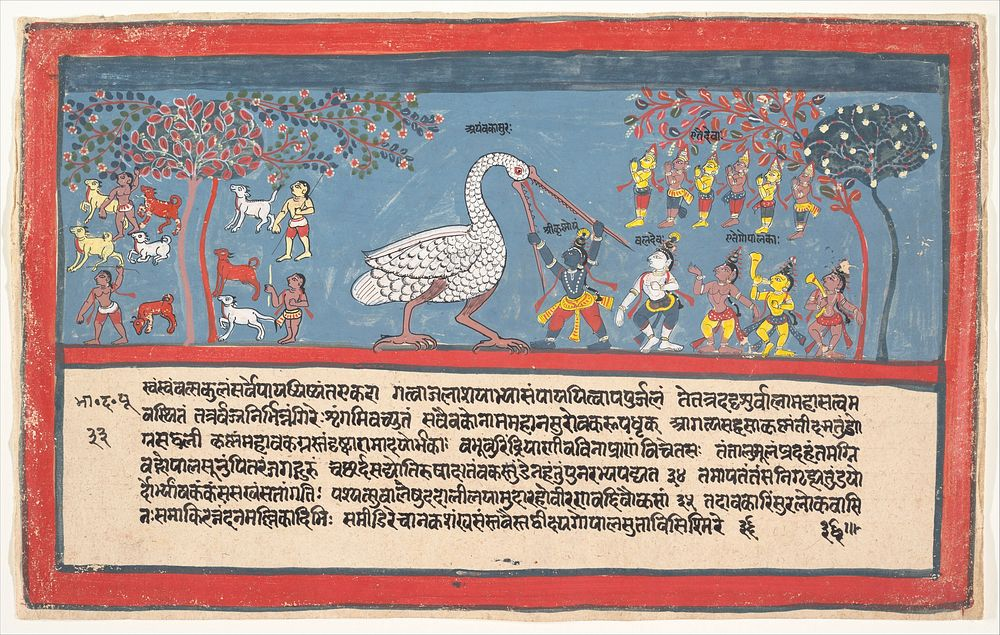
\includegraphics[width=0.8\textwidth]{puranas.jpg}
        \caption{Lord Krishna Images - Rawpixel}
      \end{figure}
    \end{column}
  \end{columns}
\end{frame}